\chapter{Collections of Data}
\label{chap:lists}
F\# is tuned to work with collections of data, and there are several built-in types of collections with various properties making them useful for different tasks. Examples include strings, lists, and arrays. Strings were discussed in \Cref{chap:calculator} and will be revisited here in more details.
%Sequences will not be discussed,\jon{Should we discuss sequences?} and we will concentrate on lists and one- and two-dimensional arrays.

The data structures discussed below all have operators, properties, methods, and modules to help you write elegant programs using them.

Properties and methods are common object-oriented terms used in conjunction with the discussed functionality. They are synonymous with values and functions and will be discussed in \Cref{chap:oop}. Properties and methods for a value or variable are called using the \idx{dot notation}, i.e., with the \lexeme{.}-lexeme. For example, \lstinline{"abcdefg".Length} is a property and is equal to the length of the string, and \lstinline|"abcdefg".ToUpper()| is a method and creates a new string where all characters have been converted to upper case.

The data structures also have accompanying modules with a wealth of functions and where some are mentioned here. Further, the data structures are all implemented as classes offering even further functionality. The modules are optimized for functional programming, see \Crefrange{sec:recursion}{chap:functional}, while classes are designed to support object-oriented programming, see \Crefrange{chap:oop}{chap:oopp}.

In the following, a brief overview of many properties, methods, and functions is given by describing their name and type-definition, and by giving a short description and an example of their use. Several definitions are general and works with many different types. To describe this we will use the notation of generic types, see \Cref{sec:functions}. The name of a generic type starts with the \lexeme{'} lexeme, such as \lstinline{'T}. The implication of the appearance of a generic type in, e.g., a function's type-definition, is that the function may be used with any real type such as \lstinline{int} or \lstinline{char}. If the same generic type name is used in several places in the type-definition, then the function must use a real type consistently. For example, The \lstinline{List.fromArray} function has type \lstinline{arr:'T [] -> 'T list}, meaning that it takes an array of some type and returns a list of the same type.

See the F\# Language Reference at \url{https://docs.microsoft.com/en-us/dotnet/fsharp/} for a full description of all available functionality including variants of those included here.

\section{Strings}
\label{sec:strings}
Strings have been discussed in \Cref{chap:calculator}, the content of which will be briefly revisited here followed by a description of some of the many supporting built-in functions in F\# on strings.

A \idx{string} is a sequence of characters. Each character is represented using UTF-16, see \Cref{sec:characterSets} for further details on the unicode standard. The type \lstinline{string} is an alias for \idx[System.string@\lstinline{System.string}]{\lstinline{System.string}}. String literals are delimited by double quotation marks \lexeme{"} and inside the delimiters, character escape sequences are allowed (see \Cref{tab:escapeChar}), which are replaced by the corresponding character code. Examples are \lstinline{"This is a string"}, \lstinline{"\tTabulated string"}, \lstinline{"A \"quoted\" string"}, and \lstinline{""}. Strings may span several lines, and new lines inside strings are part of the string unless the line is ended with a backslash. Strings may be \idx[verbatim string]{verbatim} by preceding the string with \lexeme{@}, in which case escape sequences are not replaced, but two double quotation marks are an escape sequence which is replaced by a one double quotation mark. Examples of \lexeme{@}-verbatim strings are: \lstinline{@"This is a string"}, \lstinline{@"\tNon-tabulated string"}, \lstinline{@"A ""quoted"" string"}, and \lstinline{@""}. Alternatively, a verbatim string may be delimited by three double quotation marks. Examples of \lexeme{"""}-verbatim strings are: \lstinline{"""This is a string"""}, \lstinline{"""\tNon-tabulated string"""}, \lstinline{"""A "quoted" string"""}, and \lstinline{""""""}. Strings may be indexed using the \lstinline{.[]} notation, as demonstrated in \Cref{stringIndexing}.

\subsection{String Properties and Methods}
Strings have a few properties which are values attached to each string and accessed using the \lexeme{.} notation. The only to be mentioned here is:
\begin{description}
\item[\texttt{IndexOf()}:] \lstinline{str:string -> int}. Returns the index of the first occurence of \lstinline{s} or $-1$, if \lstinline{str} does not appear in the string.
  \fsOutput{stringIndexOfMethod}{\lstinline{IndexOf()}}\idxss{IndexOf@\lstinline{IndexOf}}
\item[\texttt{Length}:] \lstinline{int}. Returns the length of the string.
  \fsOutput{stringLengthProp}{\lstinline{Length}}\idxss{Length@\lstinline{Length}}
\item[\texttt{ToLower()}:] \lstinline{unit -> string}. Returns a copy of the string where each letter has been converted to lower case.
  \fsOutput{stringToLowerMethod}{\lstinline{ToLower()}}\idxss{ToLower@\lstinline{ToLower}}
\item[\texttt{ToUpper()}:] \lstinline{unit -> string}. Returns a copy of the string where each letter has been converted to upper case.
  \fsOutput{stringToUpperMethod}{\lstinline{ToUpper()}}\idxss{ToUpper@\lstinline{ToUpper}}
\item[\texttt{Trim()}:] \lstinline{unit -> string}. Returns a copy of the string where leading and trailing whitespaces have been removed.
  \fsOutput{stringTrimMethod}{\lstinline{Trim()}}\idxss{Trim@\lstinline{Trim}}
\item[\texttt{Split()}:] \lstinline{unit -> string []}. Splits a string of words separated by spaces into an array of words. See \Cref{sec:arrays} for more information about arrays.
  \fsOutput{stringSplitMethod}{\lstinline{Split()}}\idxss{Split@\lstinline{Split}}
\end{description}

\subsection{The String Module}
The \lstinline{String} module offers many functions for working with strings. Some of the most powerful ones are listed below, and they are all higher-order functions.
\begin{description}
\item[\texttt{String.collect}:] \lstinline{f:(char -> string) -> str:string -> string}. Creates a new string whose characters are the results of applying \lstinline{f} to each of the characters of \lstinline{str} and concatenating the resulting strings.
   \fsOutput{stringCollect}{\lstinline{String.collect}}\idxss{String.collect@\lstinline{String.collect}}
% \item[\texttt{String.concat}:] \lstinline{string -> seq<string> -> string}. Returns a new string made by concatenating the given strings with a separator. Here \lstinline{seq<string>} is a sequence but can also be a list or an array. 
% \fsOutput{stringConcat}{\lstinline{String.concat}}\idxss{String.concat@\lstinline{String.concat}}
 \item[\texttt{String.exists}:] \lstinline{f:(char -> bool) -> str:string -> bool}. Returns true if any character in \lstinline{str} evaluates to true when using \lstinline{f}.
  \fsOutput{stringExists}{\lstinline{String.exists}}\idxss{String.exists@\lstinline{String.exists}}
 \item[\texttt{String.forall}:] \lstinline{f:(char -> bool) -> str:string -> bool}. Returns true if all characters in \lstinline{str} evalutes to true when using \lstinline{f}.
 \fsOutput{stringForall}{\lstinline{String.forall}}\idxss{String.forall@\lstinline{String.forall}}
\item[\texttt{String.init}:] \lstinline{n:int -> f:(int -> string) -> string}. Creates a new string with length \lstinline{n} and whose characters are the result of applying \lstinline{f} to each index of that string.
\fsOutput{stringInit}{\lstinline{String.init}}\idxss{String.init@\lstinline{String.init}}
\item[\texttt{String.iter}:] \lstinline{f:(char -> unit) -> str:string -> unit}. Applies \lstinline{f} to each character in \lstinline{str}.
\fsOutput{stringIter}{\lstinline{String.iter}}\idxss{String.iter@\lstinline{String.iter}}
% \item[\texttt{String.iteri}:] \lstinline{(int -> char -> unit) -> string -> unit}. Applies a specified function to the index of each character in the string and the character itself.
% \fsOutput{stringIterI}{\lstinline{String.iteri}}\idxss{String.iteri@\lstinline{String.iteri}}
% \item[\texttt{String.length}:] \lstinline{string -> int}. Returns the length of the string.
% \fsOutput{stringLength}{\lstinline{String.length}}\idxss{String.length@\lstinline{String.length}}
 \item[\texttt{String.map}:] \lstinline{f:(char -> char) -> str:string -> string}. Creates a new string whose characters are the results of applying \lstinline{f} to each of the characters of \lstinline{str}.
 \fsOutput{stringMap}{\lstinline{String.map}}\idxss{String.map@\lstinline{String.map}}
% \item[\texttt{String.mapi}:] \lstinline{(int -> char -> char) -> string -> string}. Creates a new string whose characters are the results of applying a specified function to each character and index of the input string.
% \fsOutput{stringMapI}{\lstinline{String.mapi}}\idxss{String.mapi@\lstinline{String.mapi}}
% \item[\texttt{String.replicate}:] \lstinline{int -> string -> string}. Returns a string by concatenating a specified number of instances of a string.
% \fsOutput{stringReplicate}{\lstinline{String.replicate}}\idxss{String.replicate@\lstinline{String.replicate}}
\end{description}

\section{Lists}
\idx[list]{Lists} are unions of immutable values of the same type. A list can be expressed as a \idx{sequence expression},
%
\begin{verbatimwrite}{\ebnf/lists.ebnf}
[[*<*expr*>{*; <*expr*>*}*]]
\end{verbatimwrite}
\syntax{\ebnf/lists.ebnf}{The syntax for a list using the sequence expression.}
%
Examples are a list of integers \mbox{\lstinline![1; 2; 3]!}, a list of strings \mbox{\lstinline!["This"; "is"; "a"; "list"]!}, a list of anonymous functions \mbox{\lstinline![(fun x -> x); (fun x -> x*x)]!}, and an empty list \lstinline![]!. Lists may also be given as ranges,
%
\begin{verbatimwrite}{\ebnf/listsRange.ebnf}
[<*expr*> .. <*expr*> [*.. <*expr*>*]]
\end{verbatimwrite}
\syntax{\ebnf/listsRange.ebnf}{The syntax for a list using the range expressions.}
%
where \lstinline[language=syntax]{<*expr*>} in \idx{range expressions} must be of integers, floats, or characters. Examples are \mbox{\lstinline![1 .. 5]!}, \mbox{\lstinline![-3.0 .. 2.0]!}, and \mbox{\lstinline!['a' .. 'z']!}. Range expressions may include a step size, thus, \mbox{\lstinline![1 .. 2 .. 10]!} evaluates to \mbox{\lstinline![1; 3; 5; 7; 9]!}.

A list type is identified with the \idx[list@\keyword{list}]{\keyword{list}} keyword, such that a list of integers has the type \lstinline!int list!. Like strings, lists may be indexed using the \idx[{.[]}@\lstinline{.[]}]{\lexeme{.[]}} notation, the lengths of lists is retrieved using the \idx[Length@\lstinline{Length}]{\lstinline{Length}} property, and we may test whether a list is empty by using the \idx[isEmpty@\lstinline{isEmpty}]{\lstinline{isEmpty}} property. These features are demonstrated in \Cref{listIndexing}.
%
\fs{listIndexing}{Lists are indexed as strings and has a \lstinline{Length} property.}
%
F\# implements lists as linked lists, as illustrated in \Cref{fig:linkedList}.
\begin{figure}
  \centering
  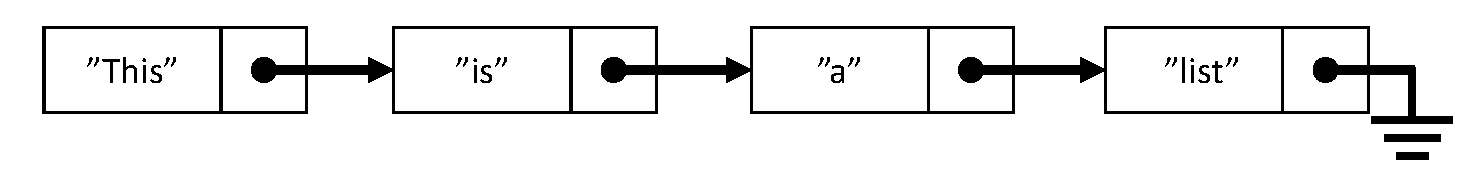
\includegraphics[width=0.75\textwidth]{linkedList}
  \caption{A list is a linked list: Here is illustrated the linked list of \mbox{\lstinline!["This"; "is"; "a"; "list"]!}.}
  \label{fig:linkedList}
\end{figure}
As a consequence, indexing element $i$ has \idx{computational complexity} $\mathcal{O}(i)$. The computational complexity of an operation is a description of how long a computation will take without considering the hardware it is performed on. The notation is sometimes called \idx{Big-O} notation or \idx{Landau notation}. In the present case, the complexity is $\mathcal{O}(i)$, which means that the complexity is linear in $i$ and indexing element $i+1$ takes $1$ unit longer than indexing element $i$ when $i$ is very large. The size of the unit is on purpose unspecified and depends on implementation and hardware details. Nevertheless, Big-O notation is a useful tool for reasoning about the efficiency of an operation. F\# has access to the list's elements only by traversing the list from its beginning. I.e., to obtain the value of element $i$, F\# starts with element 0, follows the link to element 1 and so on, until element $i$ is reached. To reach element $i+1$ instead, we would need to follow 1 more link, and assuming that following a single link takes some constant amount of time we find that the computational complexity is $\mathcal{O}(i)$.
Compared to arrays, to be discussed below, this is slow, which is why \advice{indexing lists should be avoided.}

Notice especially that lists are zero-indexed, and thus, the last element in a list \lstinline{lst} is \lstinline{lst.Length -1}. This is a very common source of error! Therefore, indexing in lists using \idx{for}-loops is supported using a special notation with the \idx[in@\lstinline{in}]{\keyword{in}} keyword,
\begin{verbatimwrite}{\ebnf/forLoopIn.ebnf}
for <*ident*> in <*list*> do <*bodyExpr*> [*done*]
\end{verbatimwrite}
\syntax{\ebnf/forLoopIn.ebnf}{For-in loop with in expression.}
In \keyword{for}-\keyword{in} loops, the loop runs through each element of the \lstinline[language=syntax]{<*list*>}, and assigns it to the identifier \lstinline[language=syntax]{<*ident*>}. This is demonstrated in \Cref{listFor}.
%
\fs{listFor}{The \keyword{for}-\keyword{in} loops are preferred over \keyword{for}-\keyword{to} loops.}
%
Using \keyword{for}-\keyword{in}-expressions remove the risk of off-by-one indexing errors, and thus, \advice{\keyword{for}-\keyword{in} is to be preferred over \keyword{for}-\keyword{to}.}

Lists support slicing identically to strings, as demonstrated in \Cref{listSlicing}.
%
\fsOutput{listSlicing}{Examples of list slicing. Compare with \Cref{stringIndexing}.}
%

Lists may be concatenated using either the \idx[{@}@{\lstinline{@}}]{\lexeme{@}}\jon{why does the at-symbol not appear in the index?} \idx[list concatenation]{concatenation} operator or the \idx[::@\lstinline{::}]{\lexeme{::}} \idx[list cons]{cons} operators. The difference is that \lexeme{@} concatenates two lists of identical types, while \lexeme{::} concatenates an element and a list of identical types.  This is demonstrated in \Cref{listCon}.
%
\fsOutput{listCon}{Examples of list concatenation.}
%
Since lists are represented as linked lists, the cons operator is very efficient and has computational complexity $\mathcal{O}(1)$, while concatenation has computational complexity $\mathcal{O}(n)$, where $n$ is the length of the first list.


It is possible to make multidimensional lists as lists of lists, as shown in \Cref{listMultidimensional}. 
%
\fs{listMultidimensional}{A ragged multidimensional list, built as lists of lists, and its indexing.}
%
The example shows a \idx{ragged multidimensional list}, since each row has a different number of elements. This is also illustrated in \Cref{fig:raggedLinkedList}.
\begin{figure}
  \centering
  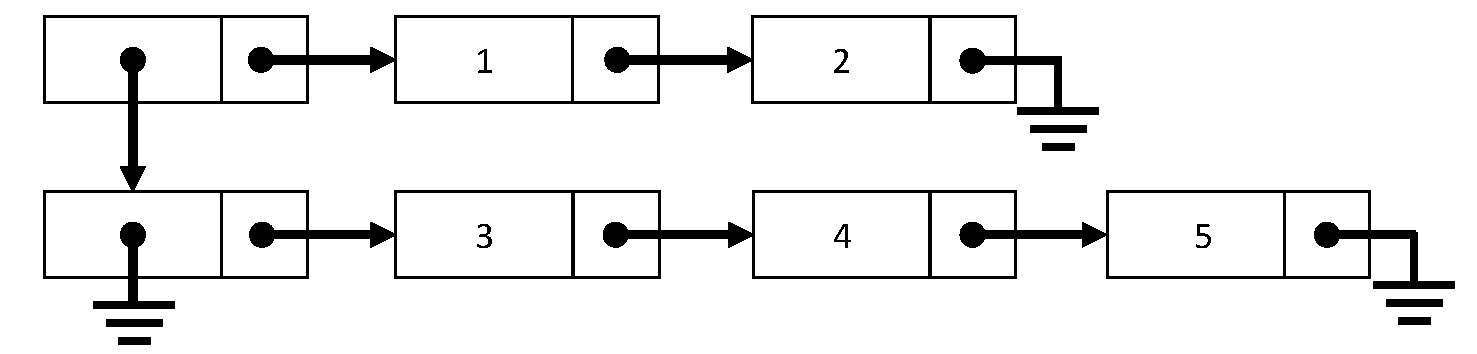
\includegraphics[width=0.75\textwidth]{raggedLinkedList}
  \caption{A list is a ragged linked list: Here is illustrated the linked list of \mbox{\lstinline![[1;2];[3;4;5]]!}.}
  \label{fig:raggedLinkedList}
\end{figure}

 The indexing of a particular element is slow due to the linked list implementation of lists, which is why arrays are often preferred for two- and higher-dimensional data structures, see \Cref{sec:arrays}.

\subsection{List Properties}
Lists support a number of properties, some of which are listed below.
\begin{description}
\item[\texttt{Head}:] Returns the first element of a list.
  \fsOutput{listHeadProp}{\lstinline{Head}}\idxss{Head@\lstinline{Head}}
\item[\texttt{IsEmpty}:] Returns true if the list is empty.
  \fsOutput{listIsEmptyProp}{\lstinline{Head}}\idxss{IsEmpty@\lstinline{IsEmpty}}
\item[\texttt{Length}:] Returns the number of elements in the list.
  \fsOutput{listLengthProp}{\lstinline{Length}}\idxss{Length@\lstinline{Length}}
\item[\texttt{Tail}:] Returns the list, except for its first element.
  \fsOutput{listTailProp}{\lstinline{Tail}}\idxss{Head@\lstinline{Tail}}
\end{description}

\subsection{The List Module}
The built-in \lstinline{List} module contains a wealth of functions for lists, some of which are
%including \lstinline!List.length!, \lstinline!List.isEmpty!, \lstinline!List.item!, \lstinline!List.head!, \lstinline!List.tail! for working with list. 
%The basic properties and members of lists are 
briefly summarized below:
%\Cref{tab:list,tab:listCont}.\idxss{Length}\idxss{List.Empty}\idxss{IsEmpty}\idxss{Item}\idxss{Head}\idxss{Tail}\idxss{Cons}
\begin{description}
\item[\texttt{List.collect}:] \lstinline{f:('T -> 'U list) -> lst:'T list -> 'U list}. Applies \lstinline{f} to each element in \lstinline{lst} and return a concatenated list of the results.
  \fsOutput{listCollect}{\lstinline{List.collect}}\idxss{List.collect@\lstinline{List.collect}}
\item[\texttt{List.contains}:] \lstinline{elm:'T -> lst:'T list -> bool}. Returns true or false depending on whether or not \lstinline{elm} is contained in \lstinline{lst}.
  \fsOutput{listContains}{\lstinline{List.contains}}\idxss{List.contains@\lstinline{List.contains}}
%\item[\texttt{List.empty}:]  \lstinline{'T list}. An empty list of inferred type.
%  \fsOutput{listEmpty}{\lstinline{List.empty}}\idxss{List.empty@\lstinline{List.empty}}
% \item[\texttt{List.exists}:] \lstinline{('T -> bool) -> 'T list -> bool}. Returns true or false depending on whether any element is true for a given function.
%   \fsOutput{listExists}{\lstinline{List.exists}}\idxss{List.exists@\lstinline{List.exists}}
\item[\texttt{List.filter}:] \lstinline{f:('T -> bool) -> lst:'T list -> 'T list}. Returns a new list with all the elements of \lstinline{lst} for which \lstinline{f} evaluates to true.
  \fsOutput{listFilter}{\lstinline{List.filter}}\idxss{List.filter@\lstinline{List.filter}}
\item[\texttt{List.find}:] \lstinline{f:('T -> bool) -> lst:'T list -> 'T}. Returns the first element of \lstinline{lst} for which \lstinline{f} is true.
  \fsOutput{listFind}{\lstinline{List.find}}\idxss{List.find@\lstinline{List.find}}
\item[\texttt{List.findIndex}:] \lstinline{f:('T -> bool) -> lst:'T list -> int}. Returns the index of the first element of \lstinline{lst} for which \lstinline{f} is true.
  \fsOutput{listFindIndex}{\lstinline{List.findIndex}}\idxss{List.findIndex@\lstinline{List.findIndex}}
\item[\texttt{List.fold}:] \lstinline{f:('State -> 'T -> 'State) -> elm:'State -> lst:'T list -> 'State}. Updates an accumulator iteratively by applying \lstinline{f} to each element in \lstinline{lst}. The initial value of the accumulator is \lstinline{elm}. For example, when \lstinline{lst} consists of \lstinline{n+1} elements
  % \lstinline{[x}$_0$\lstinline{; x}$_1$\lstinline{; x}$_2$\lstinline{;} $\ldots$\lstinline{; x}$_n$\lstinline{]}, a supplied function \lstinline{f}, and an initial value for the accumulator \lstinline{elm},
  \lstinline{List.fold} calculates:
  \begin{quote}
    \lstinline{f (}$\ldots$ \lstinline{(f (f elm lst.[0]) lst.[1])} $\ldots$\lstinline{) lst.[n]}.
  \end{quote}
  \fsOutput{listFold}{\lstinline{List.fold}}\idxss{List.fold@\lstinline{List.fold}}
\item[\texttt{List.foldBack}:] \lstinline{f:('T -> 'State -> 'State) -> lst:'T list -> elm:'State -> 'State}. Updates an accumulator iteratively backwards by applying \lstinline{f} to each element in \lstinline{lst}. The initial value of the accumulator is \lstinline{elm}. For exampel, when \lstinline{lst} consists of \lstinline{n+1} elements
  %function to each element in a list, e.g., for a list consisting of $x_0, x_1, x_2, \ldots, x_n$, a supplied function $f$, and an initial value for the accumulator $s$, \lstinline{List.foldBack} calculates $f(x_0, f(x_1, f(x_2, \ldots, f(x_n, s))))$.
  \lstinline{List.foldBack} calculates:
  \begin{quote}
    \lstinline{f lst.[0] (f lst.[1]} ($\ldots$\lstinline{(f lst.[n] elm)} $\ldots$\lstinline{))}.
  \end{quote}
  \fsOutput{listFoldBack}{\lstinline{List.foldBack}}\idxss{List.foldBack@\lstinline{List.foldBack}}
\item[\texttt{List.forall}:] \lstinline{f:('T -> bool) -> lst:'T list -> bool}. Returns true if all elements in \lstinline{lst} are true when \lstinline{f} is applied to them.
  \fsOutput{listForall}{\lstinline{List.forall}}\idxss{List.forall@\lstinline{List.forall}}
\item[\texttt{List.head}:] \lstinline{lst:'T list -> int}. Returns the first element in \lstinline{lst}. An exception is raised if \lstinline{lst} is empty. See \Cref{sec:exceptions} for more on exceptions.
  \fsOutput{listHeadAlt}{\lstinline{List.head}}\idxss{List.head@\lstinline{List.head}}
\item[\texttt{List.init}:] \lstinline{m:int -> f:(int -> 'T) -> 'T list}. Create a list with \lstinline{m} elements and whose value is the result of applying \lstinline{f} to the index of the element.
  \fsOutput{listInit}{\lstinline{List.init}}\idxss{List.init@\lstinline{List.init}}
\item[\texttt{List.isEmpty}:]  \lstinline{lst:'T list -> int}. Returns true if \lstinline{lst} is empty.
  \fsOutput{listIsEmptyAlt}{\lstinline{List.isEmpty}}\idxss{List.isEmpty@\lstinline{List.isEmpty}}
% \item[\texttt{List.item}:]  \lstinline{'T list -> int}. Retrieves an element of a list by its index.
%   \fsOutput{listItemAlt}{\lstinline{List.item}}\idxss{List.item@\lstinline{List.item}}
\item[\texttt{List.iter}:] \lstinline{f:('T -> unit) -> lst:'T list -> unit}. Applies \lstinline{f} to every element in \lstinline{lst}.
  \fsOutput{listIter}{\lstinline{List.iter}}\idxss{List.iter@\lstinline{List.iter}}
% \item[\texttt{List.Length}:]  \lstinline{'T list -> int}. Returns the number of elements in a list.
%   \fsOutput{listLengthAlt}{\lstinline{List.Length}}\idxss{List.Length@\lstinline{List.Length}}
\item[\texttt{List.map}:] \lstinline{f:('T -> 'U) -> lst:'T list -> 'U list}. Returns a list as a concatenation of applying \lstinline{f} to every element of \lstinline{lst}.
  \fsOutput{listMap}{\lstinline{List.map}}\idxss{List.map@\lstinline{List.map}}
\item[\texttt{List.ofArray}:] \lstinline{arr:'T [] -> 'T list}. Returns a list whose elements are the same as \lstinline{arr}. See \Cref{sec:arrays} for more on arrays.
  \fsOutput{listOfArray}{\lstinline{List.ofArray}}\idxss{List.ofArray@\lstinline{List.ofArray}}
\item[\texttt{List.rev}:] \lstinline{lst:'T list -> 'T list}. Returns a new list with the same elements as in \lstinline{lst} but in reversed order.
  \fsOutput{listRev}{\lstinline{List.rev}}\idxss{List.rev@\lstinline{List.rev}}
\item[\texttt{List.sort}:] \lstinline{lst:'T list -> 'T list}. Returns a new list with the same elements as in \lstinline{lst} but where the elements are sorted.
  \fsOutput{listSort}{\lstinline{List.sort}}\idxss{List.sort@\lstinline{List.sort}}
\item[\texttt{List.tail}:]  \lstinline{'T list -> 'T list}. Returns a new list identical to \lstinline{lst} but without its first element. An Exception is raised if \lstinline{lst} is empty.  See \Cref{sec:exceptions} for more on exceptions.
  \fsOutput{listTailAlt}{\lstinline{List.tail}}\idxss{List.tail@\lstinline{List.tail}}
\item[\texttt{List.toArray}:] \lstinline{lst:'T list -> 'T []}. Returns an array whose elements are the same as \lstinline{lst}.  See \Cref{sec:arrays} for more on arrays.
  \fsOutput{listToArray}{\lstinline{List.toArray}}\idxss{List.toArray@\lstinline{List.toArray}}
\item[\texttt{List.unzip}:] \lstinline{lst:('T1 * 'T2) list -> 'T1 list * 'T2 list}. Returns a pair of lists of all the first elements and all the second elements of \lstinline{lst}, respectively.
  \fsOutput{listUnzip}{\lstinline{List.unzip}}\idxss{List.unzip@\lstinline{List.unzip}}
\item[\texttt{List.zip}:] \lstinline{lst1:'T1 list -> lst2:'T2 list -> ('T1 * 'T2) list}. Returns a list of pairs, where elements in \lstinline{lst1} and \lstinline{lst2} are iteratively paired.
  \fsOutput{listZip}{\lstinline{List.zip}}\idxss{List.zip@\lstinline{List.zip}}
\end{description}

\section{Arrays}
\label{sec:arrays}
One dimensional \idx{arrays}, or just arrays for short, are mutable lists of the same type and follow a similar syntax as lists. Arrays can be stated as a \idx{sequence expression},
%
\begin{verbatimwrite}{\ebnf/arrays.ebnf}
[|[*<*expr*>{*; <*expr*>*}*]|]
\end{verbatimwrite}
\syntax{\ebnf/arrays.ebnf}{The syntax for an array using the sequence expression.}
%
Examples are arrays of integers \mbox{\lstinline![|1; 2; 3|]!}, of strings \mbox{\lstinline![|"This"; "is"; "an"; "array"|]!}, of functions \mbox{\lstinline![|(fun x -> x); (fun x -> x*x)|]!}, and an empty array \lstinline![||]!.  Arrays may also be given as ranges,
%
\begin{verbatimwrite}{\ebnf/arrayRange.ebnf}
[|<*expr*> .. <*expr*> [*.. <*expr*>*]|]
\end{verbatimwrite}
\syntax{\ebnf/arrayRange.ebnf}{The syntax for an array using the range expression.}
%
but arrays of \idx{range expressions} must be of \lstinline[language=syntax]{<*expr*>} integers, floats, or characters. Examples are \mbox{\lstinline![|1 .. 5|]!}, \mbox{\lstinline![|-3.0 .. 2.0|]!}, and \mbox{\lstinline![|'a' .. 'z'|]!}. Range expressions may include a step size, thus, \mbox{\lstinline![|1 .. 2 .. 10|]!} evaluates to \mbox{\lstinline![|1; 3; 5; 7; 9|]!}.

The array type is defined using the \keyword{array} keyword or alternatively the \lexeme{[]} lexeme.  Like strings and lists, arrays may be indexed using the \idx[{.[]}@\lstinline{.[]}]{\lexeme{.[]}} notation. Arrays cannot be resized, but are mutable, as shown in \Cref{arrayReassign}.
%
\fs{arrayReassign}{Arrays are mutable in spite of the missing \keyword{mutable} keyword.}
%
Notice that in spite of the missing \keyword{mutable} keyword, the function \lstinline{square} still has the \idx{side-effect} of squaring all entries in \lstinline{A}.  F\# implements arrays as chunks of memory and indexes arrays via address arithmetic. I.e., element $i$ in an array, whose first element is in memory address $\alpha$ and whose elements fill $\beta$ addresses each, is found at address $\alpha+i\beta$.\jon{Add a figure illustrating address indexing.} Hence, indexing has computational complexity of $\mathcal{O}(1)$, but appending and prepending values to arrays and array concatenation requires copying the new and existing values to a fresh area in memory and thus has computational complexity $\mathcal{O}(n)$, where $n$ is the total number of elements. Thus, \advice{indexing arrays is fast, but cons and concatenation is slow and should be avoided.}

Arrays support \idx{slicing}, that is, indexing an array with a range result in a copy of the array with values corresponding to the range. This is demonstrated in \Cref{arraySlicing}.
%
\fsOutput{arraySlicing}{Examples of array slicing. Compare with \Cref{listSlicing} and \Cref{stringIndexing}.}
%
As illustrated, the missing start or end index imply from the first or to the last element, respectively.

Arrays do not have explicit operator support for appending and concatenation, instead the \lstinline{Array} namespace includes an \lstinline{Array.append} function, as shown in \Cref{arrayAppend}.
%
\fs{arrayAppend}{Two arrays are appended with \lstinline{Array.append}.}
%

Arrays are \idx{reference types}, meaning that identifiers are references and thus suffer from aliasing, as illustrated in \Cref{arrayAliasing}.
%
\fs{arrayAliasing}{Arrays are reference types and suffer from aliasing.}
%

\subsection{Array Properties and Methods}
\label{sec:arrayMethods}
Some important properties and methods for arrays are:
\begin{description}
\item[\texttt{Clone()}:] \lstinline{'T []}. Returns a copy of the array.
  \fsOutput{arrayCloneProp}{\lstinline{Clone}}\idxss{Clone@\lstinline{Clone}}
\item[\texttt{Length}:] \lstinline{int}. Returns the number of elements in the array.
  \fsOutput{arrayLengthProp}{\lstinline{Length}}\idxss{Length@\lstinline{Length}}
\end{description}

\subsection{The Array Module}
There are quite a number of built-in procedures for arrays in the \lstinline{Array} module, some of which are summarized below.
\begin{description}
\item[\texttt{Array.append}:] \lstinline{arr1:'T [] -> arr2:'T [] -> 'T []}. Creates an new array whose elements are a concatenated copy of \lstinline{arr1} and \lstinline{arr2}.
  \fsOutput{arrayAppendAlt}{\lstinline{Array.append}}\idxss{Array.append@\lstinline{Array.append}}
% \item[\texttt{Array.compareWith}:] \lstinline{f:('T -> 'T -> int) -> arr1:'T [] -> arr2:'T [] -> int}. Traverseses \lstinline{arr1} and \lstinline{arr2} in parallel evaluating \lstinline{f} on pairs of their elements. Compares two arrays using the given comparison function, element by element.
%   \fsOutput{arrayComparewith}{\lstinline{Array.compareWith}}\idxss{Array.compareWith@\lstinline{Array.compareWith}}
%\item[\texttt{Array.concat}:] \lstinline{seq<'T []> -> 'T []}. Creates an array that contains the elements of each of the supplied sequence of arrays.
%  \fsOutput{arrayConcat}{\lstinline{Array.concat}}\idxss{Array.concat@\lstinline{Array.concat}}
\item[\texttt{Array.contains}:] \lstinline{elm:'T -> arr:'T [] -> bool}. Returns true if \lstinline{arr} contains \lstinline{elm}.
  \fsOutput{arrayContains}{\lstinline{Array.contains}}\idxss{Array.contains@\lstinline{Array.contains}}
%\item[\texttt{Array.copy}:] \lstinline{'T [] -> 'T []}. Creates an array that contains the elements of the supplied array.
%  \fsOutput{arrayCopy}{\lstinline{Array.copy}}\idxss{Array.copy@\lstinline{Array.copy}}
%\item[\texttt{Array.create}:] \lstinline{n:int -> v:'T -> 'T []}. Creates an array of length \lstinline{n} with value \lstinline{v}.
%  \fsOutput{arrayCreate}{\lstinline{Array.create}}\idxss{Array.create@\lstinline{Array.create}}
%\item[\texttt{Array.empty}:] \lstinline{'T []}. Creates an empty array of the given type.
%  \fsOutput{arrayEmpty}{\lstinline{Array.empty}}\idxss{Array.empty@\lstinline{Array.empty}}
\item[\texttt{Array.exists}:] \lstinline{f:('T -> bool) -> arr:'T [] -> bool}. Returns true if any application of \lstinline{f} evaluates to true when applied to the elements of \lstinline{arr}.
  \fsOutput{arrayExists}{\lstinline{Array.exists}}\idxss{Array.exists@\lstinline{Array.exists}}
%\item[\texttt{Array.fill}:] \lstinline{'T [] -> int -> int -> 'T -> unit}. Fills a range of elements of an array with the supplied value.
%  \fsOutput{arrayFill}{\lstinline{Array.fill}}\idxss{Array.fill@\lstinline{Array.fill}}
\item[\texttt{Array.filter}:] \lstinline{f:('T -> bool) -> arr:'T [] -> 'T []}. Returns an array of elements from \lstinline{arr} who evaluate to true when \lstinline{f} is applied to them.
  \fsOutput{arrayFilter}{\lstinline{Array.filter}}\idxss{Array.filter@\lstinline{Array.filter}}
\item[\texttt{Array.find}:] \lstinline{f:('T -> bool) -> arr:'T [] -> 'T}. Returns the first element in \lstinline{arr} for which \lstinline{f} evaluates to true. The \lstinline{System.Collections.Generic.KeyNotFoundException} exception is raised if no element is found.  See \Cref{sec:exceptions} for more on exceptions.
  \fsOutput{arrayFind}{\lstinline{Array.find}}  \idxss{Array.find@\lstinline{Array.find}}
\item[\texttt{Array.findIndex}:] \lstinline{f:('T -> bool) -> arr:'T [] -> int}. Returns the index of the first element in in \lstinline{arr} for which \lstinline{f} evaluates to true. If none are found, then the \lstinline{System.Collections.Generic.KeyNotFoundException} exception is raised.  See \Cref{sec:exceptions} for more on exceptions.
  \fsOutput{arrayFindindex}{\lstinline{Array.findIndex}}\idxss{Array.findIndex@\lstinline{Array.findIndex}}
\item[\texttt{Array.fold}:] \lstinline{f:('State -> 'T -> 'State) -> elm:'State -> arr:'T [] -> 'State}. Updates an accumulator iteratively by applying \lstinline{f} to each element in \lstinline{arr}. The initial value of the accumulator is \lstinline{elm}. For example, when \lstinline{arr} consists of \lstinline{n+1} elements
  \lstinline{Array.fold} calculates:
  \begin{quote}
    \lstinline{f (}$\ldots$ \lstinline{(f (f elm arr.[0]) arr.[1])} $\ldots$\lstinline{) arr.[n]}.
  \end{quote}
  \fsOutput{arrayFold}{\lstinline{Array.fold}}\idxss{Array.fold@\lstinline{Array.fold}}
\item[\texttt{Array.foldBack}:] \lstinline{f:('T -> 'State -> 'State) -> arr:'T [] -> elm:'State -> 'State}. Updates an accumulator iteratively backwards by applying \lstinline{f} to each element in \lstinline{arr}. The initial value of the accumulator is \lstinline{elm}. For exampel, when \lstinline{arr} consists of \lstinline{n+1} elements
  %function to each element in a list, e.g., for a list consisting of $x_0, x_1, x_2, \ldots, x_n$, a supplied function $f$, and an initial value for the accumulator $s$, \lstinline{List.foldBack} calculates $f(x_0, f(x_1, f(x_2, \ldots, f(x_n, s))))$.
  \lstinline{List.foldBack} calculates:
  \begin{quote}
    \lstinline{f arr.[0] (f arr.[1]} ($\ldots$\lstinline{(f arr.[n] elm)} $\ldots$\lstinline{))}.
  \end{quote}
  \fsOutput{arrayFoldback}{\lstinline{Array.foldBack}}\idxss{Array.foldBack@\lstinline{Array.foldBack}}
\item[\texttt{Array.forall}:] \lstinline{f:('T -> bool) -> arr:'T [] -> bool}. Returns true if \lstinline{f} evaluates to true for every element in \lstinline{arr}.
  \fsOutput{arrayForall}{\lstinline{Array.forall}}\idxss{Array.forall@\lstinline{Array.forall}}
%\item[\texttt{Array.get}:] \lstinline{'T [] -> int -> 'T}. Gets an element from an array.
%  \fsOutput{arrayGet}{\lstinline{Array.get}}\idxss{Array.get@\lstinline{Array.get}}
\item[\texttt{Array.init}:] \lstinline{m:int -> f:(int -> 'T) -> 'T []}. Create an array with \lstinline{m} elements and whose value is the result of applying \lstinline{f} to the index of the element.
  \fsOutput{arrayInit}{\lstinline{Array.init}}\idxss{Array.init@\lstinline{Array.init}}
\item[\texttt{Array.isEmpty}:] \lstinline{arr:'T [] -> bool}. Returns true if \lstinline{arr} is empty.
  \fsOutput{arrayIsempty}{\lstinline{Array.isEmpty}}\idxss{Array.isEmpty@\lstinline{Array.isEmpty}}
\item[\texttt{Array.iter}:] \lstinline{f:('T -> unit) -> arr:'T [] -> unit}. Applies \lstinline{f} to each element of \lstinline{arr}.
  \fsOutput{arrayIter}{\lstinline{Array.iter}}\idxss{Array.iter@\lstinline{Array.iter}}
%\item[\texttt{Array.length}:] \lstinline{'T [] -> int}. Returns the length of an array. The \lstinline{System.Array.Length} property does the same thing.
%  \fsOutput{arrayLength}{\lstinline{Array.length}}\idxss{Array.length@\lstinline{Array.length}}
\item[\texttt{Array.map}:] \lstinline{f:('T -> 'U) -> arr:'T [] -> 'U []}. Creates an new array whose elements are the results of applying \lstinline{f} to each of the elements of \lstinline{arr}.
  \fsOutput{arrayMap}{\lstinline{Array.map}}\idxss{Array.map@\lstinline{Array.map}}
\item[\texttt{Array.ofList}:] \lstinline{lst:'T list -> 'T []}. Creates an array whose elements are copied from \lstinline{lst}.
  \fsOutput{arrayOflist}{\lstinline{Array.ofList}}\idxss{Array.ofList@\lstinline{Array.ofList}}
\item[\texttt{Array.rev}:] \lstinline{arr:'T [] -> 'T []}. Creates a new array whose elements are identical to \lstinline{arr} but in reverse order.
  \fsOutput{arrayRev}{\lstinline{Array.rev}}\idxss{Array.rev@\lstinline{Array.rev}}
%\item[\texttt{Array.set}:] \lstinline{'T [] -> int -> 'T -> unit}. Sets an element of an array.
%  \fsOutput{arraySet}{\lstinline{Array.set}}\idxss{Array.set@\lstinline{Array.set}}
\item[\texttt{Array.sort}:] \lstinline{arr:'T[] -> 'T []}. Creates a new array with the same elements as in \lstinline{arr} but in sorted order %Sorts the elements of an array and returns a new array. \lstinline{Operators.compare} is used to compare the elements.
  \fsOutput{arraySort}{\lstinline{Array.sort}}\idxss{Array.sort@\lstinline{Array.sort}}
%\item[\texttt{Array.sub}:] \lstinline{'T [] -> int -> int -> 'T []}. Creates an array that contains the supplied subrange, which is specified by starting index and length.
%  \fsOutput{arraySub}{\lstinline{Array.sub}}\idxss{Array.sub@\lstinline{Array.sub}}
\item[\texttt{Array.toList}:] \lstinline{arr:'T [] -> 'T list}. Creates a new list whose elements are copied from \lstinline{arr}.
  \fsOutput{arrayTolist}{\lstinline{Array.toList}}\idxss{Array.toList@\lstinline{Array.toList}}
\item[\texttt{Array.unzip}:] \lstinline{arr:('T1 * 'T2) [] -> 'T1 [] * 'T2 []}. Returns a pair of arrays of all the first elements and all the second elements of \lstinline{arr}, respectively.
  \fsOutput{arrayUnzip}{\lstinline{Array.unzip}}\idxss{Array.unzip@\lstinline{Array.unzip}}
%\item[\texttt{Array.zeroCreate}:] \lstinline{int -> 'T []}. Creates an array whose elements are initially set to the default value \lstinline{Unchecked.defaultof<'T>}.
%  \fsOutput{arrayZerocreate}{\lstinline{Array.zeroCreate}}\idxss{Array.zeroCreate@\lstinline{Array.zeroCreate}}
\item[\texttt{Array.zip}:] \lstinline{arr1:'T1 [] -> arr2:'T2 [] -> ('T1 * 'T2) []}. Returns a list of pairs, where elements in \lstinline{arr1} and \lstinline{arr2} are iteratively paired.
  \fsOutput{arrayZip}{\lstinline{Array.zip}}\idxss{Array.zip@\lstinline{Array.zip}}
\end{description}

\section{Multidimensional Arrays}
\idx[multidimensional arrays]{Multidimensional arrays} can be created as arrays of arrays (of arrays \dots). These are known as \idx{jagged arrays}, since there is no inherent guarantee that all sub-arrays are of the same size. The example in \Cref{arrayJagged} is a jagged array of increasing width.
%
\fs{arrayJagged}{An array of arrays. When row lengths are of non-equal elements, then it is a jagged array.}
%
Indexing arrays of arrays is done sequentially, in the sense that in the above example, the number of outer arrays is \lstinline|a.Length|,  \lstinline|a.[i]| is the i'th array, the length of the i'th array is \lstinline|a.[i].Length|, and the j'th element of the i'th array is thus \lstinline|a.[i].[j]|. Often 2-dimensional rectangular arrays are used, which can be implemented as a jagged array, as shown in \Cref{arrayJaggedSquare}.
%
\fs{arrayJaggedSquare}{A rectangular array.} 
%
Note that the \keyword{for}-\keyword{in} cannot be used in \lstinline!pownArray!, e.g., 
\begin{quote} 
  \mbox{\lstinline{for row in arr do for elm in row do elm <- pown elm p done done}},
 \end{quote}
since the iterator value \lstinline!elm! is not mutable, even though \lstinline!arr! is an array.

Square arrays of dimensions 2 to 4 are so common that F\# has built-in modules for their support. Here, we will describe \idx[Array2D@\lstinline{Array2D}]{\lstinline{Array2D}}. The workings of \idx[Array3D@\lstinline{Array3D}]{\lstinline{Array3D}} and \idx[Array4D@\lstinline{Array4D}]{\lstinline{Array4D}} are very similar. A generic \lstinline{Array2D} has type \lstinline{'T [,]}, and it is indexed also using the \lstinline|[,]| notation. The \lstinline{Array2D.length1} and \lstinline{Array2D.length2} functions are supplied by the \lstinline{Array2D} module for obtaining the size of an array along the first and second dimension. Rewriting the with jagged array example in \Cref{arrayJaggedSquare} to use \lstinline{Array2D} gives a slightly simpler program, which is shown in \Cref{array2D}.
%
\fs{array2D}{Creating a 3 by 4 rectangular array of integers.}
%
Note that the \lstinline!printf! supports direct printing of the 2-dimensional array. \lstinline{Array2D} arrays support slicing. The \lexeme{*} lexeme is particularly useful to obtain all values along a dimension. This is demonstrated in \Cref{array2DSlicing}.
%
\fsOutput{array2DSlicing}{Examples of Array2D slicing. Compare with \Cref{array2D}.}
%
Note that in almost all cases, slicing produces a sub-rectangular 2 dimensional array, except for \lstinline{arr.[1,*]}, which is an array, as can be seen by the single \lexeme{[}. In contrast, \lstinline{A.[1..1,*]} is an Array2D. Note also that \lstinline!printfn! typesets 2 dimensional arrays as \lstinline{[[ ... ]]} and not \lstinline{[|[| ... |]|]}, which can cause confusion with lists of lists.
%\jon{Array2D.ToString produces \lstinline{[[ ... ]]} and not \lstinline{[|[| ... |]|]}, which can cause confusion.}

Multidimensional arrays have the same properties and methods as arrays, see \Cref{sec:arrayMethods}.

\subsection{The Array2D Module}
There are quite a number of built-in procedures for arrays in the \lstinline{Array2D} namespace, some of which are summarized below.\jon{rewrite description}
\begin{description}
\item[\texttt{copy}:] \lstinline{arr:'T [,] -> 'T [,]}. Creates a new array whose elements are copied from \lstinline{arr}.
  \fsOutput{array2DCopy}{\lstinline{Array2D.copy}}\idxss{Array2D.copy@\lstinline{Array2D.copy}}
\item[\texttt{create}:] \lstinline{m:int -> n:int -> v:'T -> 'T [,]}. Creates an \lstinline{m} by \lstinline{n} array whose elements are set to \lstinline{v}.
  \fsOutput{array2DCreate}{\lstinline{Array2D.create}}\idxss{Array2D.create@\lstinline{Array2D.create}}
%\item[\texttt{get}:] \lstinline{'T [,] -> int -> int -> 'T}. Fetches an element from a 2D array. You can also use the syntax \lstinline{array.[index1,index2]}.
%  \fsOutput{array2DGet}{\lstinline{Array2D.get}}\idxss{Array2D.get@\lstinline{Array2D.get}}
\item[\texttt{init}:] \lstinline{m:int -> n:int -> f:(int -> int -> 'T) -> 'T [,]}. Creates an \lstinline{m} by \lstinline{n} array whose elements are the result of applying \lstinline{f} to the index of an element.
  \fsOutput{array2DInit}{\lstinline{Array2D.init}}\idxss{Array2D.init@\lstinline{Array2D.init}}
\item[\texttt{iter}:] \lstinline{f:('T -> unit) -> arr:'T [,] -> unit}. Applies \lstinline{f} to each element of \lstinline{arr}.
  \fsOutput{array2DIter}{\lstinline{Array2D.iter}}\idxss{Array2D.iter@\lstinline{Array2D.iter}}
\item[\texttt{length1}:] \lstinline{arr:'T [,] -> int}. Returns the length the first dimension of \lstinline{arr}.
  \fsOutput{array2DLength1}{\lstinline{Array2D.length1}}\idxss{Array2D.length1@\lstinline{Array2D.length1}}
\item[\texttt{length2}:] \lstinline{arr:'T [,] -> int}. Returns the length of the second dimension of \lstinline{arr}.
  \fsOutput{array2DLength2}{\lstinline{Array2D.forall length2}}\idxss{Array2D.length2@\lstinline{Array2D.length2}}
\item[\texttt{map}:] \lstinline{f:('T -> 'U) -> arr:'T [,] -> 'U [,]}. Creates a new array whose elements are the results of applying \lstinline{f} to each of the elements of \lstinline{arr}.
  \fsOutput{array2DMap}{\lstinline{Array2D.map}}\idxss{Array2D.map@\lstinline{Array2D.map}}
%\item[\texttt{set}:] \lstinline{'T [,] -> int -> int -> 'T -> unit}. Sets the value of an element in an array. You can also use the syntax \lstinline{array.[index1,index2] <- value}.
%  \fsOutput{array2DSet}{\lstinline{Array2D.set}}\idxss{Array2D.set@\lstinline{Array2D.set}}
\end{description}

\begin{comment}
\section{Comparison}
% \begin{table}
%   \centering
%\afterpage{%
%  \clearpage% Flush earlier floats (otherwise order might not be correct)
%  \thispagestyle{empty}% empty page style (?)
  \begin{landscape}% Landscape page
    \centering % Center table
    \rowcolors{2}{oddRowColor}{evenRowColor}
    \begin{longtable}{|l|l|l|l|l|l|l|l|}
      \hline
      \rowcolor{headerRowColor} & Strings & Lists & Array & Array2D & Map & Set & Seq\\
      \hline
      {\lstinline!add : 'Key -> 'T -> Map<'Key,'T> -> Map<'Key,'T>!} & & & & & \cmark & \cmark &\\
      {\lstinline!append : 'T [] -> 'T [] -> 'T []!} & & \cmark&\cmark & & & &\cmark\\
      {\lstinline!average : 'T [] -> ^T!} & & \cmark & \cmark & & & &\cmark\\
      {\lstinline!averageBy : ('T -> ^U) -> 'T [] -> ^U!} & & \cmark & \cmark & & & &\cmark\\
      {\lstinline!base1 : 'T [,] -> int!} & & & & \cmark & & &\\
      {\lstinline!base2 : 'T [,] -> int!} & & & & \cmark & & &\\
      {\lstinline!blit : 'T [] -> int -> 'T [] -> int -> int -> unit!} & & & \cmark & \cmark & & &\\
      {\lstinline!cache : seq<'T> -> seq<'T>!} & & & & & & & \cmark\\
      {\lstinline!cast : seq<'T> -> seq<'T>!} & & & & & & & \cmark\\
      {\lstinline!choose : ('T -> 'U option) -> 'T [] -> 'U []!} & & \cmark & \cmark & & & & \cmark\\
      {\lstinline!chunkBySize : int -> 'T [] -> 'T [] []!} & & \cmark & & & & &\\
      {\lstinline!collect : ('T -> 'U []) -> 'T [] -> 'U []!} & \cmark & \cmark & \cmark & & & & \cmark\\
      {\lstinline!comparewith : ('T -> 'T -> int) -> 'T [] -> 'T [] -> int!} & & \cmark & \cmark & & & & \cmark\\
      {\lstinline!concat : seq<'T []> -> 'T []!} & \cmark & \cmark & \cmark & & & & \cmark\\
      {\lstinline!contains : 'T -> 'T [] -> bool!} & & \cmark & \cmark & & & \cmark & \cmark\\
      {\lstinline!containsKey : 'Key -> Map<'Key,'T> -> bool!} & & & & & \cmark & &\\
      {\lstinline!copy : 'T [,] -> 'T [,]!} & & & \cmark & \cmark & & &\\
      {\lstinline!count : Set<'T> -> int!} & & & & & & \cmark &\\
      {\lstinline!countBy : ('T -> 'Key) -> 'T [] -> ('Key * int) []!} & & \cmark & \cmark & & & & \cmark\\
      {\lstinline!create : int -> 'T -> 'T []!} & & & \cmark & \cmark & & &\\
      {\lstinline!createBased : int -> int -> int -> int -> 'T -> 'T [,]!} & & &  & \cmark & & &\\
      {\lstinline!delay : (unit -> seq<'T>) -> seq<'T>!} & & & & & & & \cmark\\
      {\lstinline!difference : Set<'T> -> Set<'T> -> Set<'T>!} & & & & & & \cmark &\\
      {\lstinline!distinct : 'T -> 'T []!} & & \cmark & \cmark & & & & \cmark\\
      {\lstinline!distinctBy : ('T -> 'Key) -> seq<'T> -> seq<'T>!} & & & & & & & \cmark\\
      {\lstinline!empty : 'T []!} & & \cmark & \cmark & & \cmark & \cmark & \cmark\\
      {\lstinline!exactlyOne : seq<'T> -> 'T!} & & & & & & & \cmark\\
      {\lstinline!exists : ('T -> bool) -> 'T [] -> bool!} & \cmark & \cmark & \cmark & & \cmark & \cmark & \cmark\\
      {\lstinline!exists2 : ('T1 -> 'T2 -> bool) -> 'T1 [] -> 'T2 [] -> bool!} & & \cmark & \cmark & & & & \cmark\\
      {\lstinline!fill : 'T [] -> int -> int -> 'T -> unit!} & & & \cmark & & & &\\
      {\lstinline!filter : ('T -> bool) -> 'T [] -> 'T []!} & & \cmark & \cmark & & \cmark & \cmark & \cmark\\
      {\lstinline!find : ('T -> bool) -> 'T [] -> 'T!} & & \cmark & \cmark & & \cmark & & \cmark\\
      {\lstinline!findKey : ('Key -> 'T -> bool) -> Map<'Key,'T> -> 'Key!} & & & & & \cmark & &\\
      {\lstinline!findIndex : ('T -> bool) -> 'T [] -> int!} & & \cmark & \cmark & & & & \cmark\\
      {\lstinline!fold : ('S -> 'T -> 'S) -> 'S -> 'T [] -> 'S!} & & \cmark & \cmark & & \cmark & \cmark & \cmark\\
      {\lstinline!fold2 : ('S -> 'T1 -> 'T2 -> 'S) -> 'S -> 'T1 [] -> 'T2 [] -> 'S!} & & \cmark & \cmark & & & &\\
      {\lstinline!foldBack : ('T -> 'S -> 'S) -> 'T [] -> 'S -> 'S!} & & \cmark & \cmark & & \cmark & \cmark &\\
      {\lstinline!foldBack2 : ('T1 -> 'T2 -> 'S -> 'S) -> 'T1 [] -> 'T2 [] -> 'S -> 'S!} & & \cmark & \cmark & & & &\\
      {\lstinline!forall : ('T -> bool) -> 'T [] -> bool!} & \cmark & \cmark & \cmark & & \cmark & \cmark & \cmark\\
      {\lstinline!forall2 : ('T1 -> 'T2 -> bool) -> 'T1 [] -> 'T2 [] -> bool!} & & \cmark & \cmark & & & & \cmark\\
      {\lstinline!get : 'T [] -> int -> 'T!} & & & \cmark & \cmark & & &\\
      {\lstinline!groupBy : ('T -> 'Key) -> seq<'T> -> seq<'Key * seq<'T>>!} & & & & & & & \cmark\\
      {\lstinline!head : 'T [] -> 'T!} & & \cmark &  & & & &\\
      {\lstinline!init : int -> (int -> 'T) -> 'T []!} & \cmark & \cmark & \cmark & \cmark & & & \cmark\\
      {\lstinline!initBased : int -> int -> int -> int -> (int -> int -> 'T) -> 'T [,]!} &  &  &  & \cmark & & &\\
      {\lstinline!initInfinite : (int -> 'T) -> seq<'T>!} & & & & & & & \cmark\\
      {\lstinline!intersect : Set<'T> -> Set<'T> -> Set<'T>!} & & & & & & \cmark &\\
      {\lstinline!intersectMany : seq<Set<'T>> -> Set<'T>!} & & & & & & \cmark &\\
      {\lstinline!isEmpty : 'T [] -> bool!} & & \cmark & \cmark & & \cmark & \cmark & \cmark\\
      {\lstinline!isProperSubset : Set<'T> -> Set<'T> -> bool!} & & & & & & \cmark &\\
      {\lstinline!isProperSuperset : Set<'T> -> Set<'T> -> bool!} & & & & & & \cmark &\\
      {\lstinline!isSubset : Set<'T> -> Set<'T> -> bool!} & & & & & & \cmark &\\
      {\lstinline!isSuperset : Set<'T> -> Set<'T> -> bool!} & & & & & & \cmark &\\
      {\lstinline!iter : ('T -> unit) -> 'T [] -> unit!} & \cmark & \cmark & \cmark & \cmark & \cmark & \cmark & \cmark\\
      {\lstinline!iter2 : ('T1 -> 'T2 -> unit) -> 'T1 [] -> 'T2 [] -> unit!} & & \cmark & \cmark & & & & \cmark\\
      {\lstinline!iteri : (int -> 'T -> unit) -> 'T [] -> unit!} & \cmark & \cmark & \cmark & \cmark & & & \cmark\\
      {\lstinline!iteri2 : (int -> 'T1 -> 'T2 -> unit) -> 'T1 [] -> 'T2 [] -> unit!} & & \cmark & \cmark & & & & \\
      {\lstinline!last : seq<'T> -> 'T!} & & &  & & & & \cmark\\
      {\lstinline!length : 'T [] -> int!} & \cmark & \cmark & \cmark & & & & \cmark\\
      {\lstinline!length1 : 'T [,] -> int!} & & &  & \cmark & & &\\
      {\lstinline!length2 : 'T [,] -> int!} & & &  & \cmark & & &\\
      {\lstinline!map : ('T -> 'U) -> 'T [] -> 'U []!} & \cmark & \cmark & \cmark & \cmark & \cmark & \cmark & \cmark\\
      {\lstinline!map2 : ('T1 -> 'T2 -> 'U) -> 'T1 [] -> 'T2 [] -> 'U []!} & & \cmark & \cmark & & & & \cmark\\
      {\lstinline!map3 : ('T1 -> 'T2 -> 'T3 -> 'U) -> 'T1 [] -> 'T2 [] -> 'T3 [] -> 'U []!} & & \cmark & \cmark & & & &\\
      {\lstinline!mapi : (int -> 'T -> 'U) -> 'T [] -> 'U []!} & \cmark & \cmark & \cmark & \cmark & & & \cmark\\
      {\lstinline!mapi2 : (int -> 'T1 -> 'T2 -> 'U) -> 'T1 [] -> 'T2 [] -> 'U []!} & & \cmark & \cmark & & & &\\
      {\lstinline!max : 'T [] -> 'T!} & & \cmark & \cmark & & & & \cmark\\
      {\lstinline!maxBy : ('T -> 'U) -> 'T [] -> 'T!} & & \cmark & \cmark & & & & \cmark\\
      {\lstinline!maxElement : Set<'T> -> 'T!} & & & & & & \cmark &\\
      {\lstinline!min : 'T [] -> 'T!} & & \cmark & \cmark & & & & \cmark\\
      {\lstinline!minBy : ('T -> 'U) -> 'T [] -> 'T!} & & \cmark & \cmark & & & & \cmark\\
      {\lstinline!minElement : Set<'T> -> 'T!} & & & & & & \cmark &\\
      {\lstinline!nth :  'T list -> int -> 'T!} & & & & \cmark & & & \cmark\\
      {\lstinline!rebase : 'T [,] -> 'T [,]!} & & & & \cmark & & &\\
      {\lstinline!ofArray : 'T [] -> 'T []!} & & \cmark & & & \cmark & \cmark & \cmark\\
      {\lstinline!ofList : 'T list -> 'T []!} & & & \cmark & & \cmark & \cmark & \cmark\\
      {\lstinline!ofSeq : seq<'T> -> 'T []!} & & \cmark & \cmark & \cmark & \cmark & &\\
      {\lstinline!partition : ('T -> bool) -> 'T [] * 'T []!} & & \cmark & \cmark & & \cmark & \cmark &\\
      {\lstinline!parwise : seq<'T> -> seq<'T * 'T>!} & & & & & & & \cmark\\
      {\lstinline!permute : (int -> int) -> 'T [] -> 'T []!} & & \cmark & \cmark & & & &\\
      {\lstinline!pick : ('T -> 'U option) -> 'T [] -> 'U!} & & \cmark & \cmark & & \cmark & & \cmark\\
      {\lstinline!readonly : seq<'T> -> seq<'T>!} & & & & & & & \cmark\\
      {\lstinline!reduce : ('T -> 'T -> 'T) -> 'T [] -> 'T!} & & \cmark & \cmark & & & & \cmark\\
      {\lstinline!reduceBack : ('T -> 'T -> 'T) -> 'T [] -> 'T!} & & \cmark & \cmark & & & &\\
      {\lstinline!remove : 'Key -> Map<'Key,'T> -> Map<'Key,'T>!} & & & & & \cmark & \cmark &\\
      {\lstinline!replicate : (int -> 'T -> 'T [])!} & \cmark & \cmark & \cmark & & & &\\
      {\lstinline!rev : 'T [] -> 'T []!} & & \cmark & \cmark & & & &\\
      {\lstinline!scan : ('S -> 'T -> 'S) -> 'S -> 'T [] -> 'S []!} & & \cmark & \cmark & & & & \cmark\\
      {\lstinline!scanBack : ('T -> 'S -> 'S) -> 'T [] -> 'S -> 'S []!} & & \cmark & \cmark & & & &\\
      {\lstinline!set : 'T [] -> int -> 'T -> unit!} & & & \cmark & \cmark & & &\\
      {\lstinline!singleton : 'T -> seq<'T>!} & & & & & & \cmark & \cmark\\
      {\lstinline!skip : int -> seq<'T> -> seq<'T>!} & & & & & & & \cmark\\
      {\lstinline!skipWhile : ('T -> bool) -> seq<'T> -> seq<'T>!} & & & & & & & \cmark\\
      {\lstinline!sort : 'T [] -> 'T []!} & & \cmark & \cmark & & & & \cmark\\
      {\lstinline!sortBy : ('T -> 'Key) -> 'T [] -> 'T []!} & & \cmark & \cmark & & & & \cmark\\
      {\lstinline!sortInPlace : ('T -> 'Key) -> 'T [] -> unit!} & & & \cmark & & & &\\
      {\lstinline!sortInPlaceWith : ('T -> 'T -> int) -> 'T [] -> unit!} & & & \cmark & & & &\\
      {\lstinline!sortWith : ('T -> 'T -> int) -> 'T [] -> 'T []!} & & \cmark & \cmark & & & &\\
      {\lstinline!sub : 'T [] -> int -> int -> 'T []!} & & & \cmark & & & &\\
      {\lstinline!sum : ^T [] -> ^T!} & & \cmark & \cmark & & & & \cmark\\
      {\lstinline!sumBy : ('T -> ^U) -> 'T [] -> ^U!} & & \cmark & \cmark & & & & \cmark\\
      {\lstinline!tail : 'T [] -> 'T []!} & & \cmark & & & & & \cmark\\
      {\lstinline!take : int -> seq<'T> -> seq<'T>!} & & & & & & & \cmark\\
      {\lstinline!takeWhile : ('T -> bool) -> seq<'T> -> seq<'T>'!} & & & & & & & \cmark\\
      {\lstinline!toArray : 'T list -> 'T []!} & & \cmark & & & \cmark & \cmark & \cmark\\
      {\lstinline!toList[] : 'T [] -> 'T []!} & & & \cmark & & \cmark & \cmark & \cmark\\
      {\lstinline!toSeq : 'T [] -> seq<'T>!} & & \cmark & \cmark & & \cmark & \cmark &\\
      {\lstinline!truncate : int -> seq<'T> -> seq<'T>!} & & & & & & & \cmark\\
      {\lstinline!tryFind : ('T -> bool) -> 'T [] -> 'T option!} & & \cmark & \cmark & & \cmark & & \cmark\\
      {\lstinline!tryFindIndex : ('T -> bool) -> 'T [] -> int option!} & & \cmark & \cmark & & & & \cmark\\
      {\lstinline!tryFindKey : ('Key -> 'T -> bool) -> Map<'Key,'T> -> 'Key option!} & & & & & \cmark & &\\
      {\lstinline!tryPick : ('T -> 'U option) -> 'T [] -> 'U option!} & & \cmark & \cmark & & \cmark & & \cmark\\
      {\lstinline!unfold : ('State -> 'T * 'State option) -> 'State -> seq<'T>!} & & & & & & & \cmark\\
      {\lstinline!where : ('T -> bool) -> seq<'T> -> seq<'T>!} & & & & & & & \cmark\\
      {\lstinline!windowed : int -> seq<'T> -> seq<'T []>!} & & & & & & & \cmark\\
      {\lstinline!union : Set<'T> -> Set<'T> -> Set<'T>!} & & & & & & \cmark &\\
      {\lstinline!unionMany : seq<Set<'T>> -> Set<'T>!} & & & & & & \cmark &\\
      {\lstinline!unzip : ('T1 * 'T2) [] -> 'T1 [] * 'T2 []!} & & \cmark & \cmark & & & &\\
      {\lstinline!unzip3 : ('T1 * 'T2 * 'T3) [] -> 'T1 [] * 'T2 [] * 'T3 []!} & & \cmark & \cmark & & & &\\
      {\lstinline!zeroCreate : int -> 'T []!} & & & \cmark & \cmark & & &\\
      {\lstinline!zeroCreateBased : int -> int -> int -> int-> 'T [,]!} & & & & \cmark & & &\\
      {\lstinline!zip : 'T1 [] -> 'T2 [] -> ('T1 * 'T2) []!} & & \cmark & \cmark & & & & \cmark\\
      {\lstinline!zip3 : 'T1 [] -> 'T2 [] -> 'T3 [] -> ('T1 * 'T2 * 'T3) []!} & & \cmark & \cmark & & & & \cmark\\
      \hline
    \end{longtable}
    \captionof{table}{Comparing Core.String, Collections.List, Collections.Array and Collections.Array2D, Collections.Set, Collections.Map, and Collections.Seq Modules}% Add 'table' caption
    \label{tab:listableComparision}
  \end{landscape}
%  \clearpage% Flush page
%}
%  \caption{Comparing listable stuff}
%  \label{tab:listableComparision}
%\end{table}
\end{comment}    
%%% Local Variables:
%%% TeX-master: "fsharpNotes"
%%% End:

